\documentclass[a4paper, 12pt, oneside, titlepage]{article} %{\parskip}
\usepackage[top=2.54cm, bottom=2.54cm, left=3cm, right=2cm]{geometry}
\usepackage[utf8]{inputenc}
\usepackage[czech]{babel}
\usepackage[T1]{fontenc}
\usepackage{graphicx}
\usepackage{booktabs}
\usepackage{tabularx}
\usepackage{array}
\usepackage{indentfirst}
\usepackage{multicol}
\usepackage{titlesec}
\usepackage{mathtools}
\usepackage{esvect}

\usepackage{url}
\usepackage{caption}
\usepackage{subfig}
\usepackage[section]{placeins}
\usepackage{pdfpages}



\hyphenation{po-ly-gon desk-to-po-vá}

\newcommand{\tg}{\mathop{\rm tg}\nolimits}
\newcommand{\arctg}{\mathop{\rm arctg}\nolimits}
\newtheorem{defin}{Definice}

\begin{document}

%\pagestyle{empty}
\setcounter{page}{1}   % nastaví čítač stránek znovu od jedné
\pagenumbering{arabic} % číslování arabskými
\thispagestyle{empty}

\begin{center}

\large

\v{C}eské vysoké učení technické v~Praze

\medskip

Fakulta stavební
\medskip

Katedra geomatiky

\vfill
\centerline{\mbox{
\includegraphics[scale=1.3]{obrazky/symbol_cvut_konturova_verze.jpg}} }


{\bf\Large Technická zpráva}

\vfill

{\bf\LARGE\bfseries Algoritmy v digitální kartografii}

\vfill

{\bf\Large Úloha č. 4: Množinové operace s polygony}


\vfill



\vfill
\vspace{5mm}

\begin{tabular}{c}

{\bf Bc. Pane Kuzmanov}\\
\noalign{\vspace{2mm}}
{\bf Bc. František Mužík}\\
\noalign{\vspace{10mm}}

Studijní program: Geodézie a kartografie \\
\noalign{\vspace{2mm}}

Specializace: Geomatika\\

\end{tabular}


\vfill

% Zde doplňte rok
Praha 2021

\end{center}

%---------------------------------------------------------------------
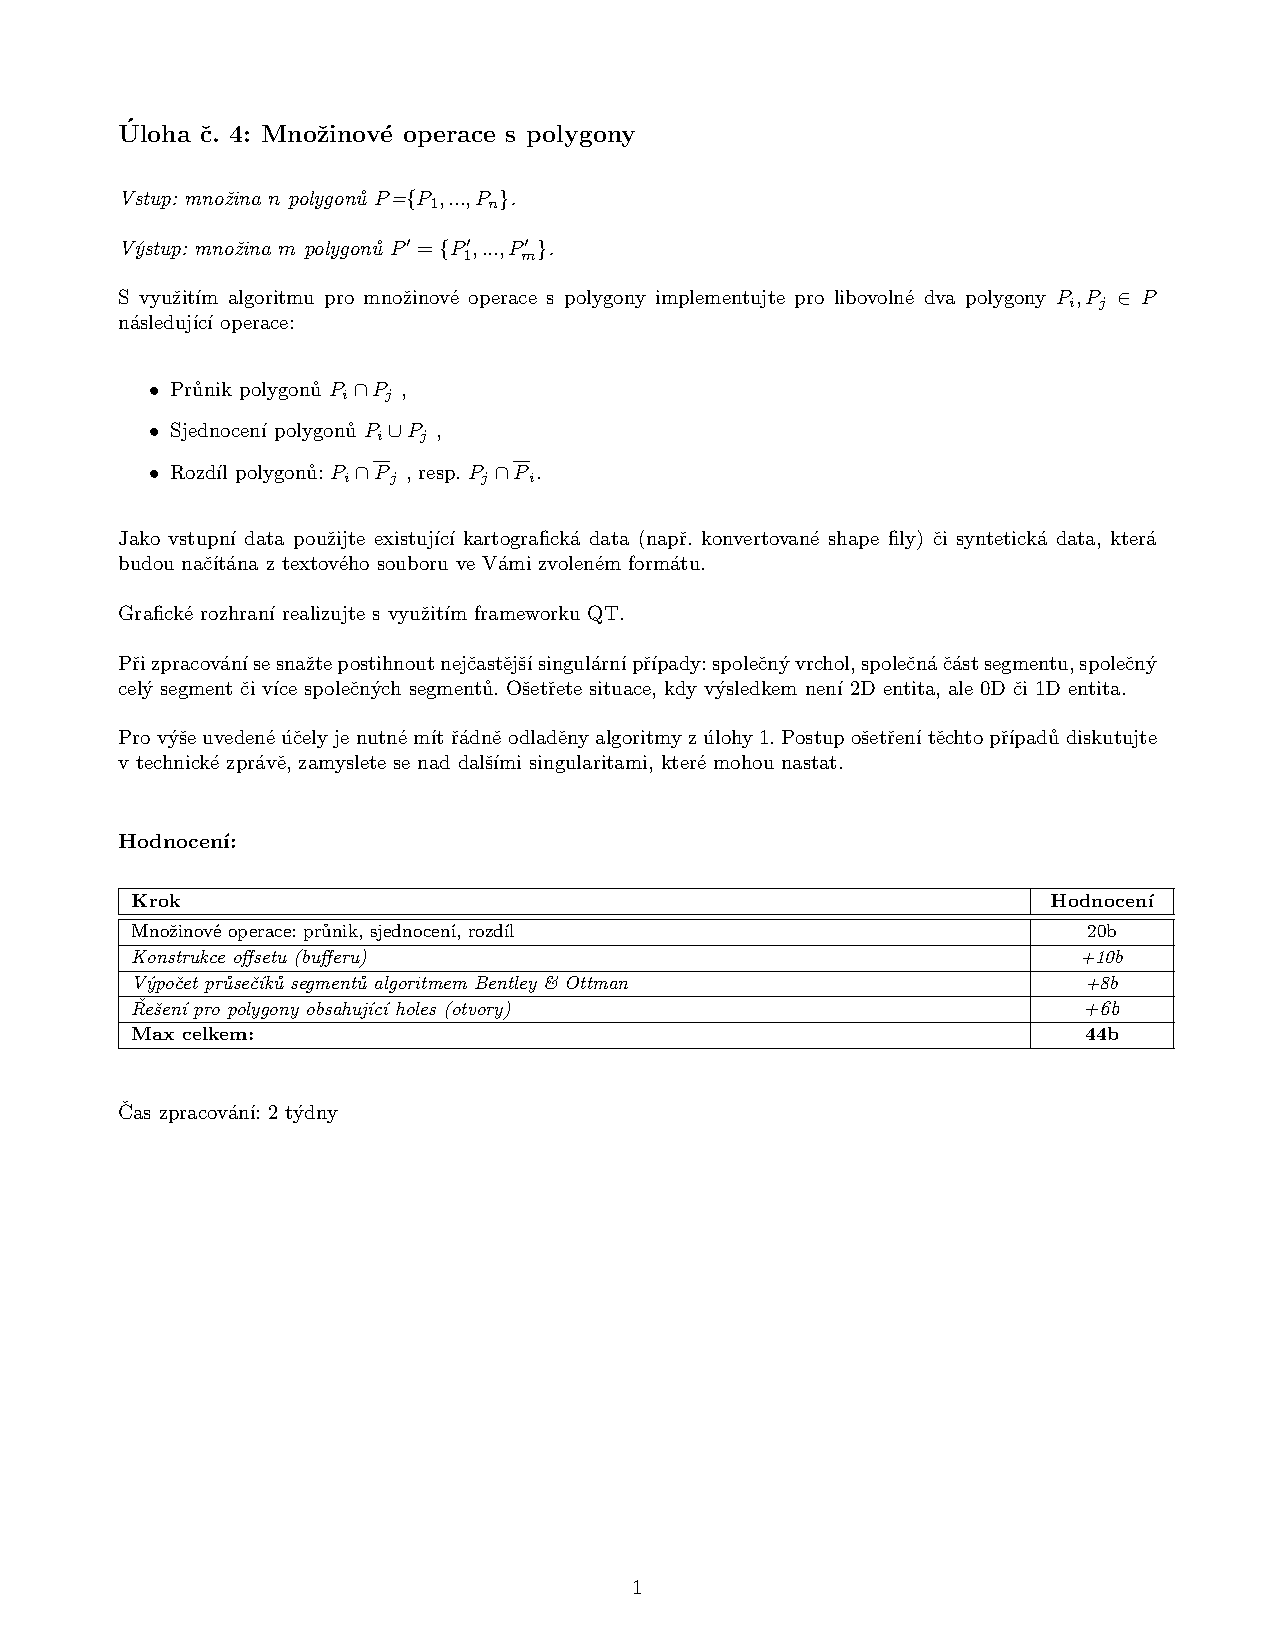
\includepdf{adkcv4}

%---------------------------------------------------------------------
\clearpage
\section{Údaje o bonusových úlohách}

\subsection{Konstrukce offsetu (bufferu) (+10b)}


\subsection{Výpočet průsečíků segmentů algoritmem Bentley \& Ottoman (+8b)}
Tato bonusová úloha nebyla řešena.

\subsection{Řešení pro polygony obsahující holes (otvory) (+6b)}
Tato bonusová úloha nebyla řešena.


\section{Popis a rozbor problému}
Nechť existují dva polygony $A,B$ tvořené body $P_1$ až $P_n$. Pro tyto polygony je potřeba zjistit jejich vzájemnou polohu užitím následujících množinových operací: průnik $A\cap B$, sjednocení $A\cup B$ a rozdíl($A-B, B-A$) (viz. obr.~\ref{fig:mn_operace}). Uživateli je zobrazen výsledek zvolené množinové operace s~využitím grafického zvýraznění částí polygonů.

Popis jednotlivých množinových operací včetně jejich implementace je podrobně rozepsán v~kapitole~\ref{popisalg}.

Při řešení problému je potřeba postihnout některé singulární případy (viz.~kapitola~\ref{problemsit}).

\begin{figure}[!htb]
	\centering
	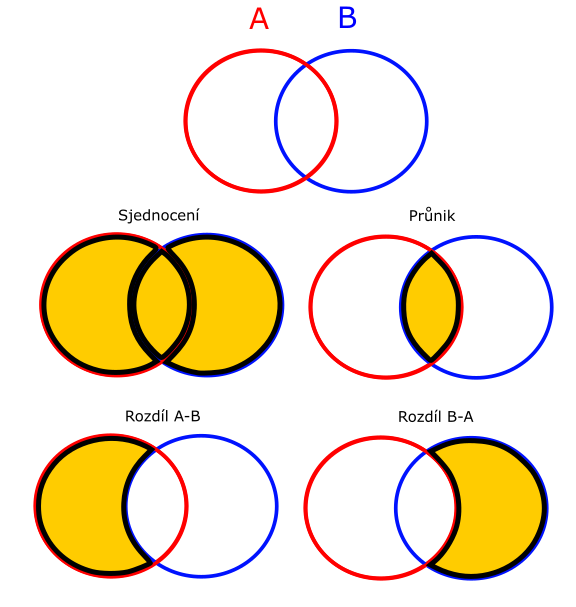
\includegraphics[scale=0.6]{obrazky/mn_operace.png} 
	\caption{Množinové operace.
	}
	\label{fig:mn_operace}
\end{figure} 
\FloatBarrier

\textbf{Popis množinových operací:}
\begin{itemize}
\item \textbf{Sjednocení:}Výsledkem je taková množina, která obsahuje každý prvek, který se nachází alespoň ~jedné ze sjednocovaných množin, a žádné další prvky.
\item \textbf{Průnik:} Výsledkem je taková množina, která obsahuje pouze ty prvky, které se nalézají v~obou množinách a obsahuje všechny takové prvky.
\item \textbf{Rozdíl:} Výsledkem je taková množina, která obsahuje každý prvek, který se nachází v~první z~množin, ale nenachází se ve druhé z~nich, a žádné další prvky. 

\end{itemize}

\section{Popisy algoritmů formálním jazykem} \label{popisalg}
\subsection{Určení polohy bodu pomocí Winding Number Algorithm} \label{winding}
Jestliže pozorovatel stojí na námi určeném bodě~$q$. Při určení polohy bodu vůči polygonu~$P$ se následně pozorovatel otáčí na bodě~$q$ proti směru hodinových ručiček. Při otočení proti směru hodinových ručiček, se úhlu přiřadí kladné znaménko a naopak, při otočení podél směru hodinových ručiček, je přiřazeno znaménko záporné. Pozorovatel takto zapisuje úhly~$\omega$ mezi jednotlivými vrcholy polygonu, dokud se nedostane do počátečního bodu. Dále se vypočte suma všech úhlů (tzv. Winding number) s~uvedením příslušných znamének a provede se určení polohy: 
\begin{itemize}
\item Pokud $q \in P$ a pozorovatel chce vidět více $\forall pi \in P$, musí se otočit o úhel 2$\pi$.
\item Pokud $q \notin P$, je tento úhel menší než 2$\pi$.
\end{itemize}


\noindent\textbf{Zadáno:} bod~$q$, polygon~$P$ tvořený vrcholy $p_i$

\noindent\textbf{Určováno:} úhly mezi vrcholy $\omega(p_i,q,p_{i+1} )$

\noindent\textbf{Implementace algoritmu:}

Ze souřadnic bodů jsou vypočteny vektory $\vec{u}_{\,i} = (q,p_i)$ a $\vec{v}_{\,i} = (q,p_{i+1})$. 

Dále probíhá výpočet jednotlivých úhlů: $\cos\omega = \dfrac{\vec{u}_{\,i}\cdot\vec{u}_{\,i}}{\vert\vec{u}_{\,i}\vert\cdot\vert\vec{v}_{\,i}\vert}$.

\begin{enumerate}
  \item Inicializace $\Omega = 0$, tolerance $\epsilon$. Natavení tolerance vychází z nutnosti porovnávání reálných, nikoliv celých, čísel.
  \item Opakování pro $\forall$ trojici $(p_i,q,p_{i+1} )$.
  \item \quad Určení polohy $q$ vzhledem k hranici polygonu $p = (p_i, p_{i+1})$. Tedy jestli bod leží vlevo, vpravo nebo na úsečce (hranici polygonu).
  \item \quad Určení úhlu $\omega_i = \angle p_i,q, p_{i+1}$.
  \item \quad Zjištění do jaké poloroviny bod patří. Pokud $q \in \overline{\Omega_l}$, pak $\Omega = \Omega + \omega_i$. Bod bude v ležet v levé polorovině.
  \item \quad Jinak $\Omega = \Omega - \omega_i$. Pak bod bude ležet v pravé polorovině. 
  \item Závěrem je proveden test na odchylku od $2\pi$. Pokud $\vert\vert\Omega\vert - 2\pi\vert < \epsilon$, pak se bod~$q$ nachází uvnitř polygonu~$P$.
  \item Jinak bod~$q$ leží mimo polygon~$P$.
\end{enumerate}

\subsection{Výpočet průsečíků polygonů A,B}
Následující algoritmus slouží k výpočtu průsečíků dvou hran polygonů A,B. Tyto průsečíky jsou ukládány do mapy s~klíčem $\alpha$, $\beta$, které určují polohu průsečíku dvou hran a hodnotou danou průsečíkem. Po nalezení každého dalšího průsečíku je mapa aktualizována a body v~ní seřazeny dle hodnot $\alpha$, $\beta$. Závěrem je s~užitím algoritmu Winding Number (viz. kapitola~\ref{winding}) určena poloha vrcholů jednoho polygonu vůči druhému (a naopak), z~čehož poté vychází výsledky jednotlivých množinových operací, jež jsou sepsány v~tabulce~\ref{tab:mnop}.

\noindent\textbf{Implementace algoritmu:}
\begin{enumerate}
\item $for(i=0; i<n; i++)$
\item \quad Vytvoření mapy: $M=map(double,QPointFBO)$
\item \quad $for(j=0; j<m; j++)$
\item \quad \quad Pokud existuje průsečík: $if b_{ij}=(p_i,p_{(i+1)\%m})\cap (q_j,q_{(j+1)\%m}) \neq 0$
\item \quad \quad \quad Přidání do mapy M: $M[\alpha_i] \leftarrow b_{ij}$
\item \quad \quad \quad Zpracování prvního průsečíku pro $e_{j}^{'}$:  $processIntersection(b_{ij}, \beta, B, j)$
\item \quad Pokud jsou nalezeny nějaké průsečíky: $if(\Vert M \Vert >0)$
\item \quad \quad Procházení všech průsečíků v~mapě: $for(\forall m\in M):$ 
\item \quad \quad \quad Získání 2. hodnoty páru: $b\leftarrow m.second$
\item \quad \quad \quad Zpracování aktuálního průsečíku pro $e_i$: $processIntersection(b, \alpha, A, i)$
\end{enumerate}

\noindent\textbf{processIntersection:}
\begin{enumerate}
\item Jestliže $\epsilon$ je minimální hodnota: $if(\vert t \vert > \epsilon~\&\&~\vert \vert t \vert -1 \vert > \epsilon):$
\item \quad Inkrementace pozice: $i \leftarrow i+1$
\item \quad Přidání průsečíku na pozici i+1: $P \leftarrow (b,i)$
\end{enumerate}

\subsection{Ohodnocení hran}
Algoritmus setEdgePositions rozděluje pozice středů hran vůči polygonu. Pro pozice bodů je využit algoritmus Winding Number (kapitola~\ref{winding}). Výsledkem je buď vnitřní (inner) nebo vnější (outer) pozice.

\noindent\textbf{Implementace algoritmu:}
\begin{enumerate}
\item $for(i=0; i<n; i++)$, kde n je počet vrcholů polygonu A
\item \quad Určení středu hrany $M(x_m, y_m)$: 
\item \quad \quad $x_m=\frac{x_i+x_{i+1}}{2}$
\item \quad \quad $y_m=\frac{y_i+y_{i+1}}{2}$
\item \quad Určení pozice vůči polygonu B: $pos=getPositionWinding(M, B)$
\item \quad Aktualizováni pozice: $A(i) \leftarrow pos$
\end{enumerate}

\subsection{Množinové operace dle polohy bodů}
\begin{table}[htbp!]
\centering
\caption{Množinové operace}
\begin{tabular}{|c|c|c|}
\hline
Operace             & \textbf{Polygon A} & \textbf{Polygon B} \\ \hline
\textbf{Sjednocení} & Vnější             & Vnější             \\ \hline
\textbf{Průnik}     & Vnitřní            & Vnitřní            \\ \hline
\textbf{Rozdíl A-B} & Vnější             & Vnitřní            \\ \hline
\textbf{Rozdíl B-A} & Vnitřní            & Vnější             \\ \hline
\end{tabular}
\label{tab:mnop}
\end{table}
\FloatBarrier

\section{Problematické situace a jejich rozbor} \label{problemsit}
Problematické situace nastávají, jestliže polygony mají společný jeden či více společných vrcholů, úseků hrany a nebo celé společné hrany. Ukázky je možné prohlédnout níže na obr.~\ref{fig:problem_sit}.

\begin{figure}[!htb]
	\centering
	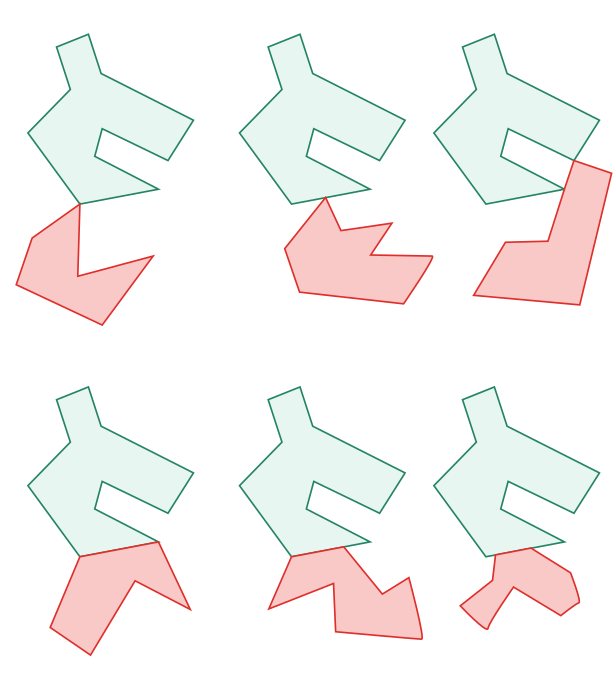
\includegraphics[scale=0.6]{obrazky/problem_sit.png} 
	\caption{Problematické situace.
	}
	\label{fig:problem_sit}
\end{figure} 
\FloatBarrier


Další problém nastává u~polygonů s~otvory. Na~obr.~\ref{fig:problem_sit_dve} je v~levé části zřetelné chybné určení sjednocení zeleného a červeného polygonu, jestliže některý polygon (zde zelený) obsahuje otvor. Vpravo je správné určení. Aplikace bohužel neumí tento problém správně vyřešit, tato bonusová úloha nebyla řešena.

\begin{figure}[!htb]
	\centering
	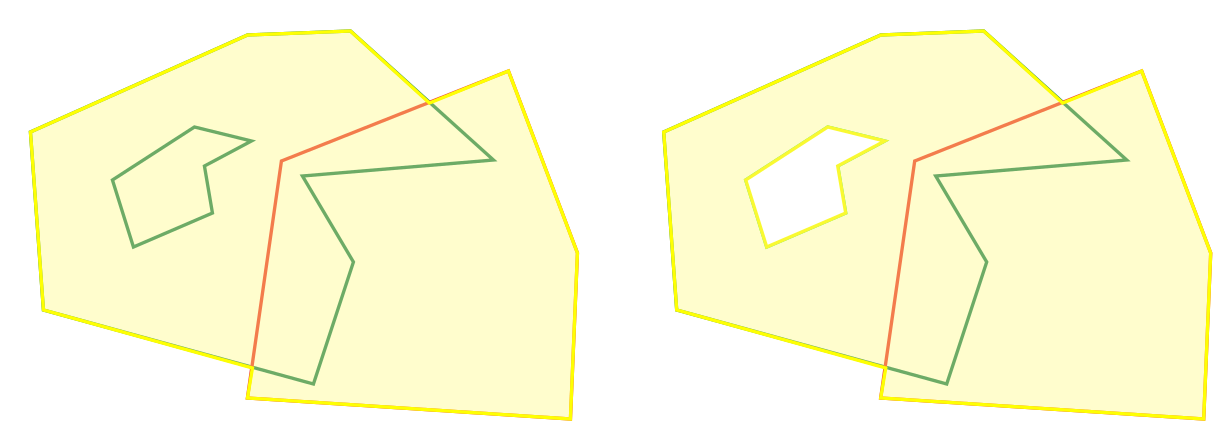
\includegraphics[scale=0.4]{obrazky/problem_sit_dve.png} 
	\caption{Problematické situace -- polygony s otvory.
	}
	\label{fig:problem_sit_dve}
\end{figure} 
\FloatBarrier

\section{Vstupní data}
% formát vstupních dat, popis
Vstupními daty je textový soubor obsahující lomové body polygonů. Jedná se o~generalizovaná data (s~tolerancí 1 km) z~datasetu ArcČR \cite{arccr}. Konkrétně jde o~Jihočeský kraj a spojené území NP a CHKO Šumava. Výběr a export dat proběhl v~softwaru ArcGIS Pro \cite{arcgispro}. Každý bod je zadaný id polygonu (Šumava či Jihočeský kraj) a souřanicemi X,Y v~modifikovaném systému JTSK:

\begin{verbatim}
1 848367 1118134
1 841874 1121052
1 839753 1118724
...
\end{verbatim}



\section{Výstupní data}
% formát výstupních dat, popis
Za výstupní data je považováno grafické rozhraní vytvořené aplikace. S~jejím využitím lze posuzovat vzájemné polohy dvou polygonů a výsledky množinových operací nad nimi.


\section{Snímky obrazovky vytvořené aplikace a její popis}\label{snimky}
Na obrázku~\ref{fig:popis_aplikace} je znázorněn popis uživatelského rozhraní aplikace v~momentu po jejím spuštění. Tlačítka mají následující využití:

\begin{enumerate}
\item Import polygon umožňuje načtení polygonů z~textového souboru
\item Pomocí Switch A/B lze změnit kreslení polygonů A nebo B
\item Combo box umožňující výběr dané množinové operace
\item Create overlay vykreslí hranice polygonu zvolené množinové operace
\item Clear overlay vymaže předchozí vykreslení
\item Clear all vymaže celé okno
\end{enumerate}

\begin{figure}[!htb]
	\centering
	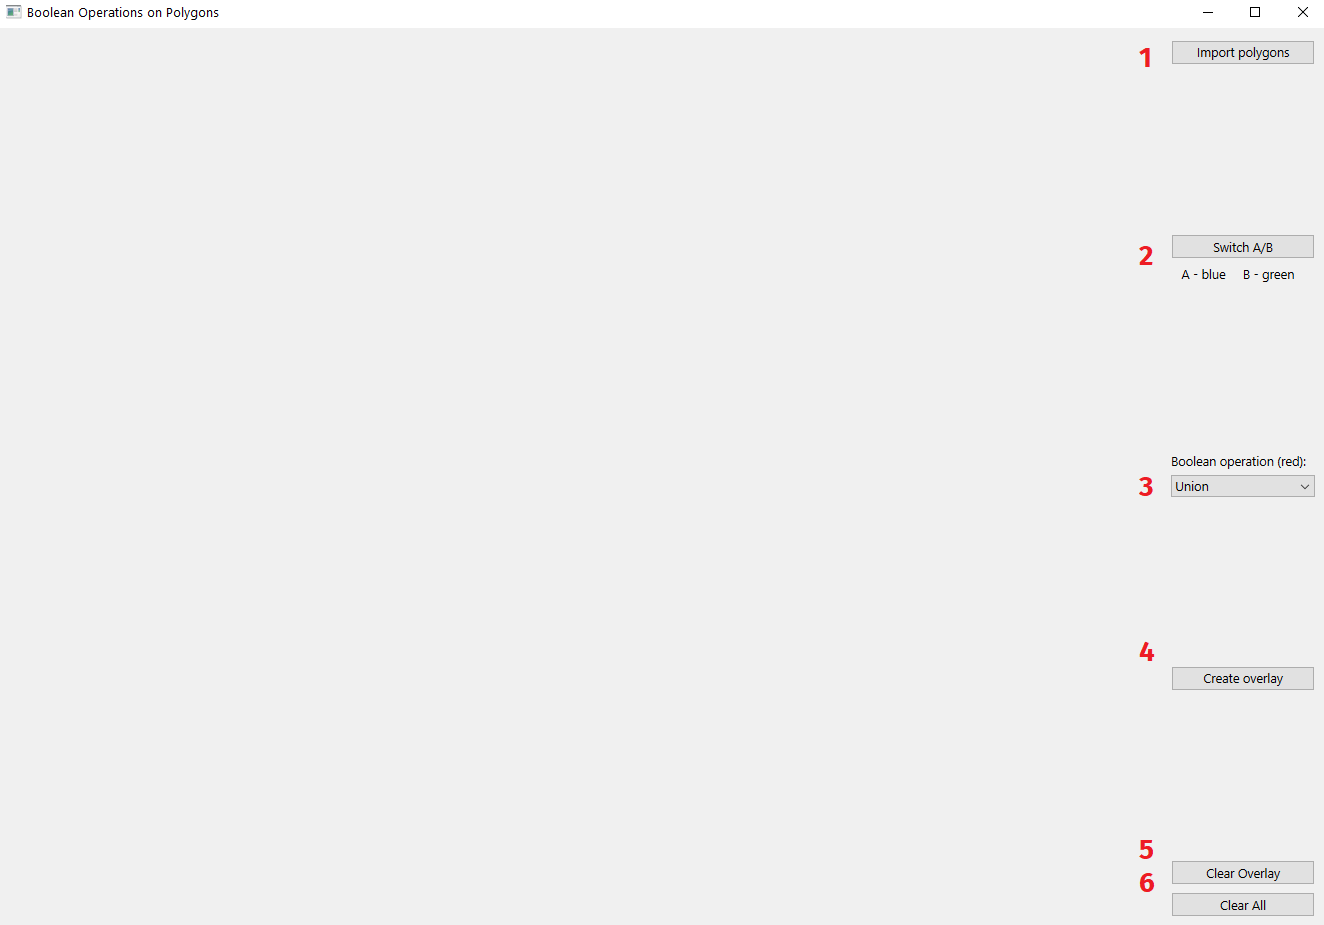
\includegraphics[scale=0.4]{obrazky/popis_aplikace.png} 
	\caption{Popis uživatelského rozhraní aplikace.
	}
	\label{fig:popis_aplikace}
\end{figure} 
\FloatBarrier


\begin{figure}[!htb]
	\centering
	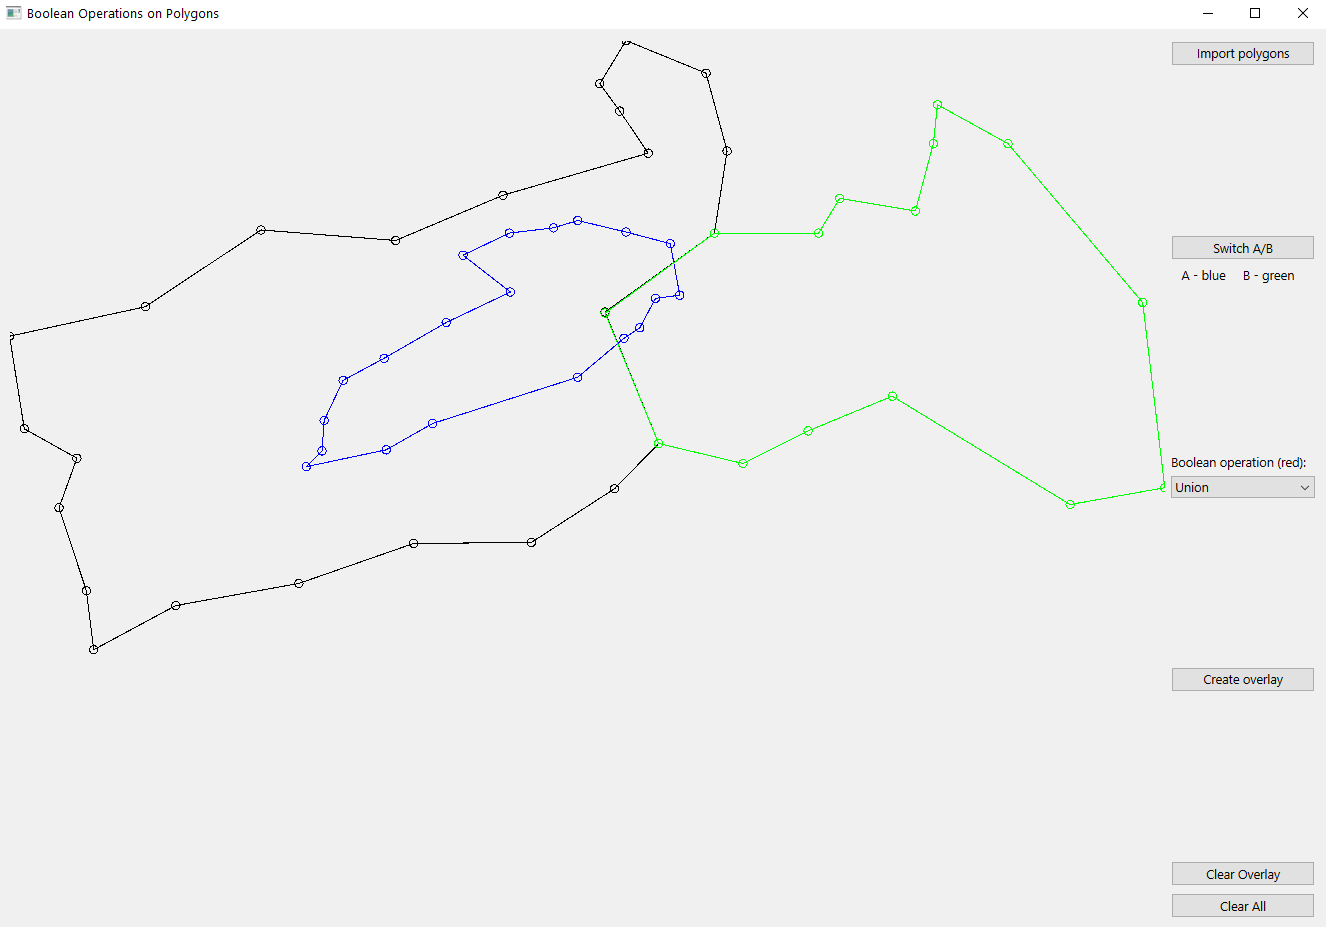
\includegraphics[scale=0.4]{obrazky/start.png} 
	\caption{Aplikace po vykreslení obou polygonů.
	}
	\label{fig:start}
\end{figure} 
\FloatBarrier

\begin{figure}[!htb]
	\centering
	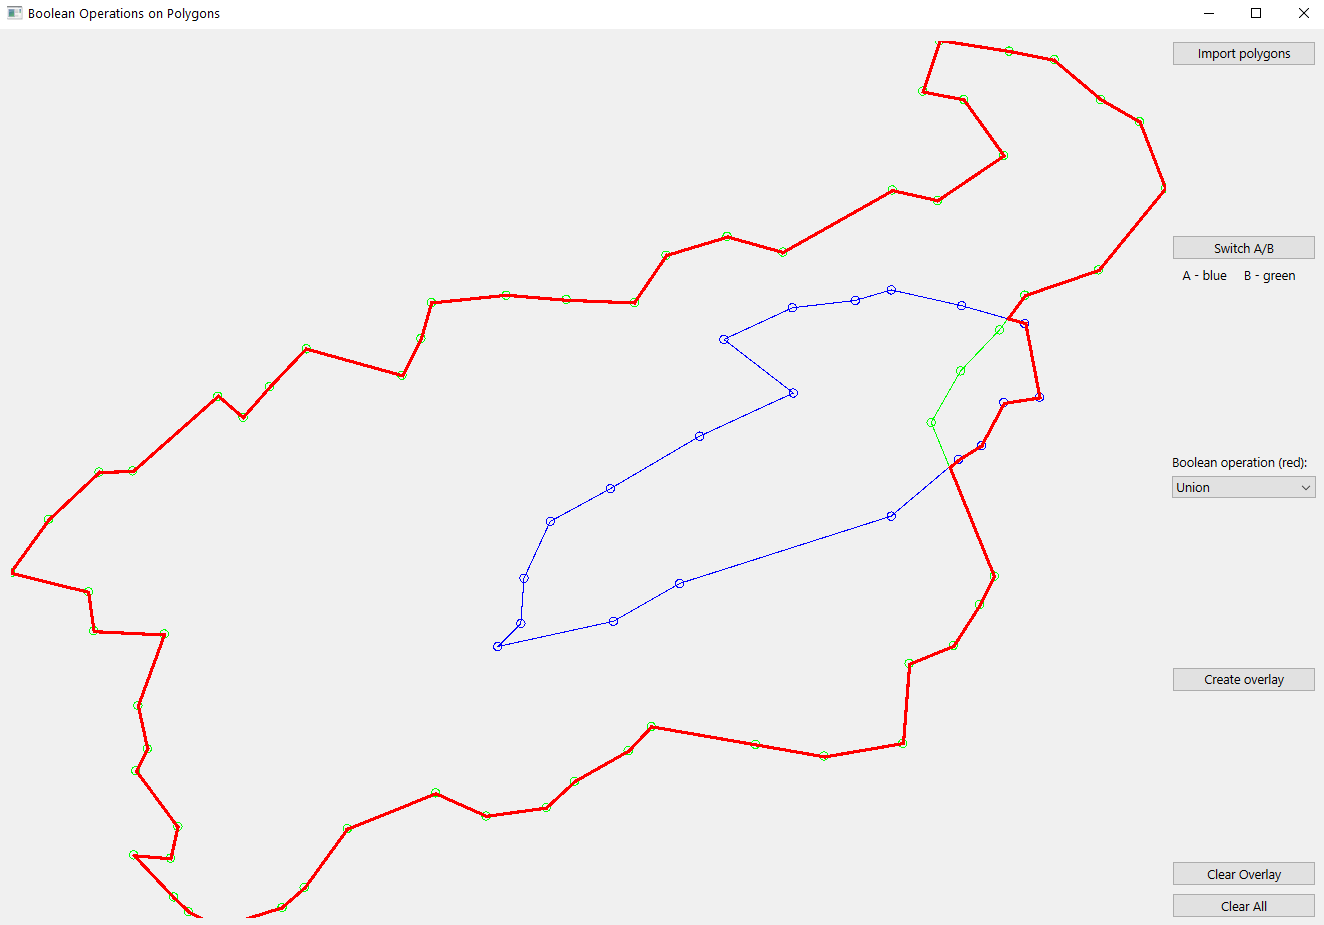
\includegraphics[scale=0.4]{obrazky/sjednoceni.png} 
	\caption{Vyhodnocení sjednocení polygonů.
	}
	\label{fig:sjednoceni}
\end{figure} 
\FloatBarrier

\begin{figure}[!htb]
	\centering
	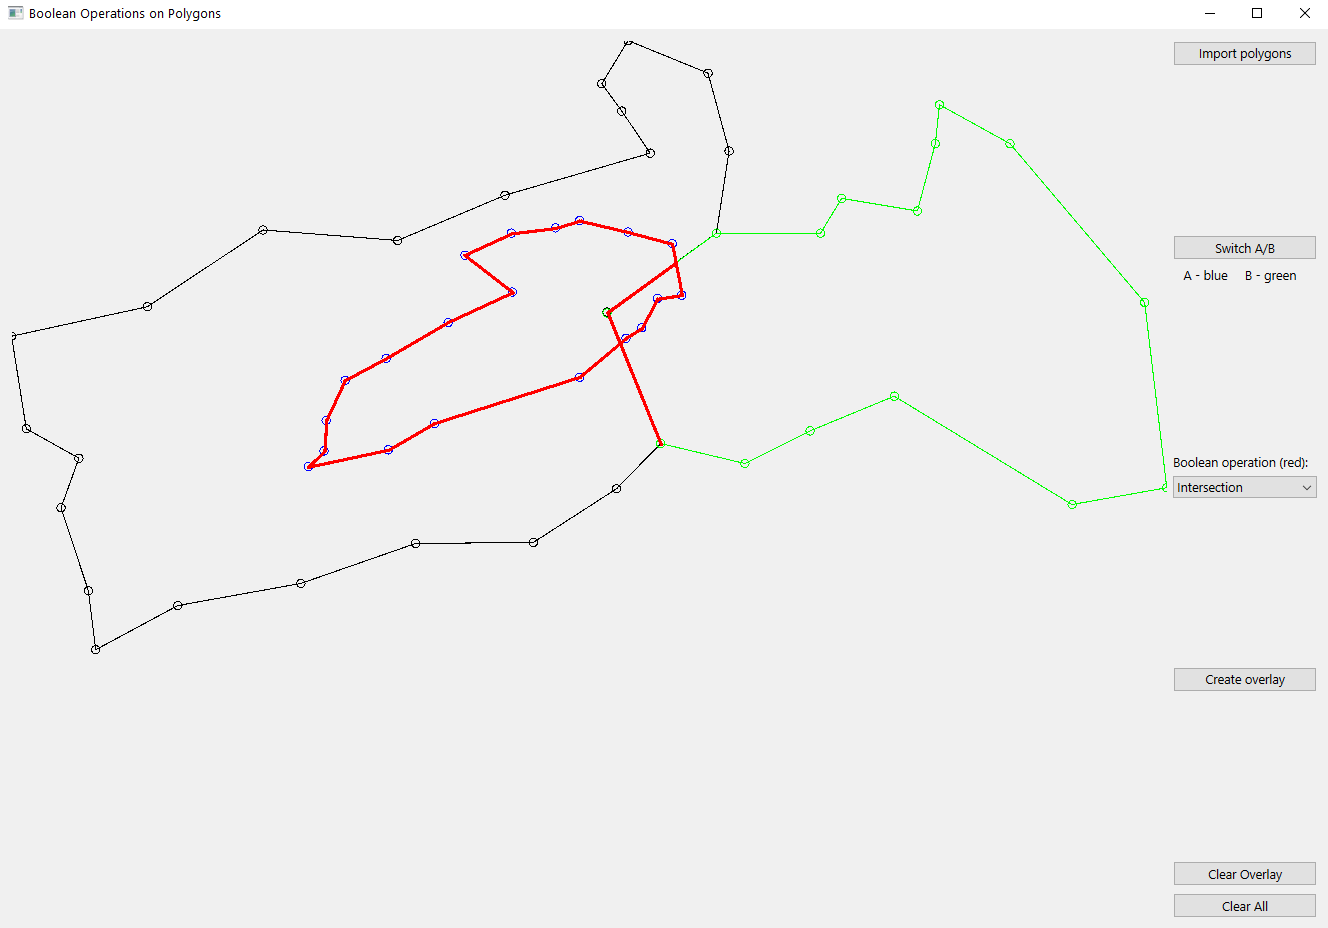
\includegraphics[scale=0.4]{obrazky/prunik.png} 
	\caption{Vyhodnocení průniku polygonů.
	}
	\label{fig:prunik}
\end{figure} 
\FloatBarrier

\begin{figure}[!htb]
	\centering
	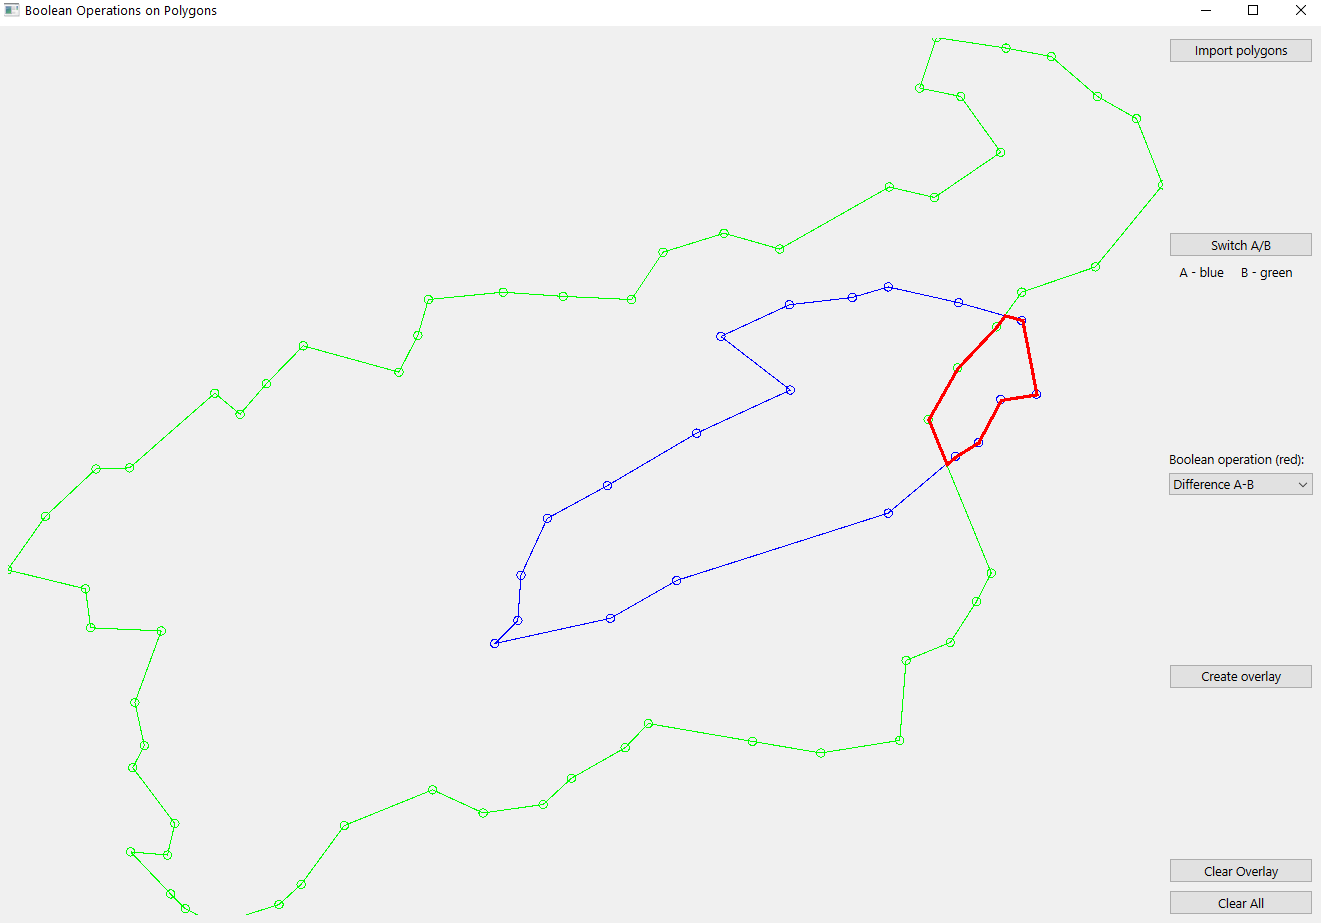
\includegraphics[scale=0.4]{obrazky/rozAB.png} 
	\caption{Vyhodnocení rozdílu polygonů A-B.
	}
	\label{fig:rozAB}
\end{figure} 
\FloatBarrier

\begin{figure}[!htb]
	\centering
	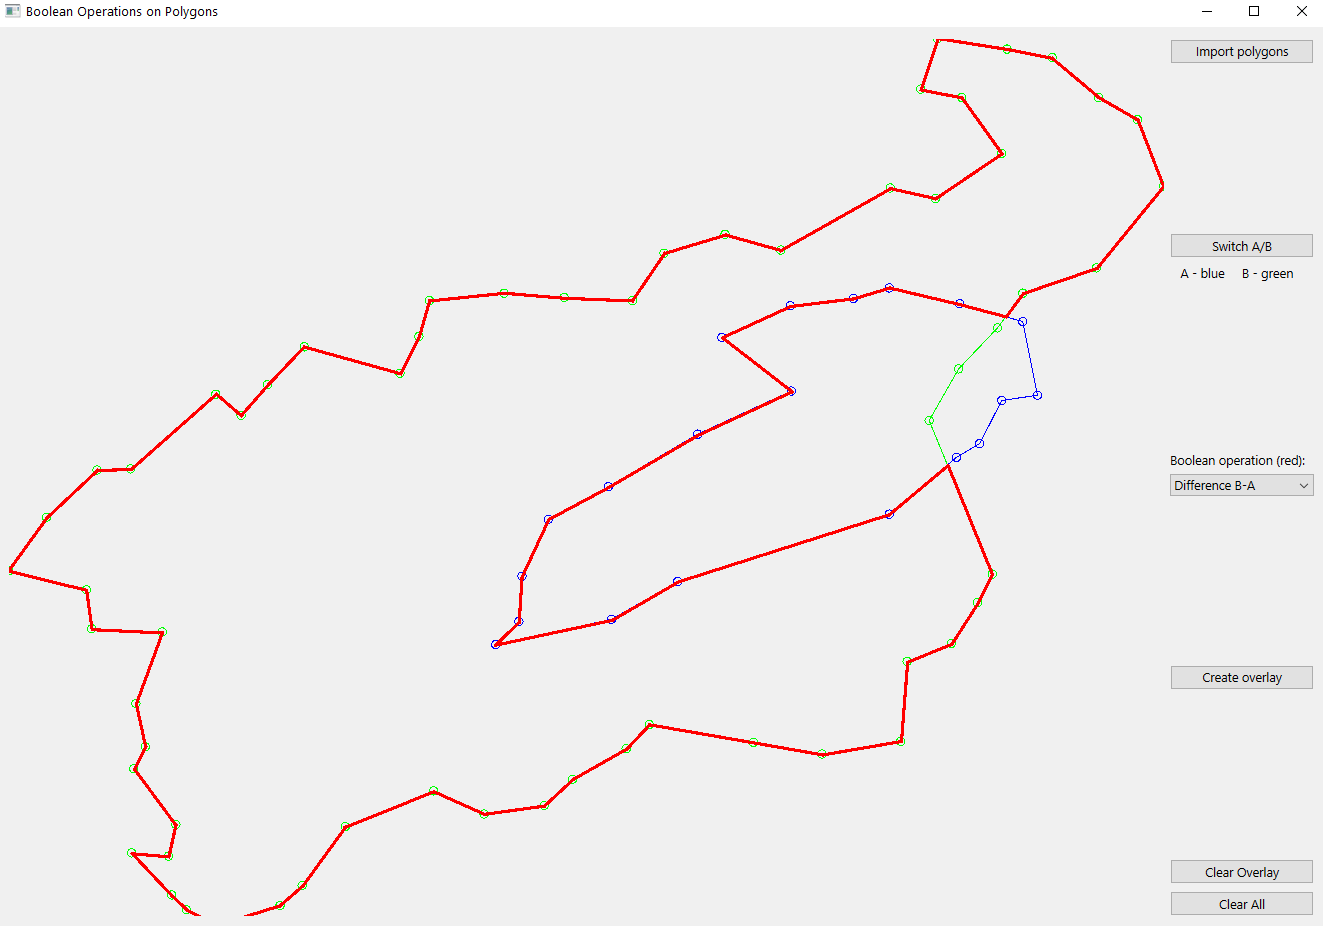
\includegraphics[scale=0.4]{obrazky/rozBA.png} 
	\caption{Vyhodnocení rozdílu polygonů B-A.
	}
	\label{fig:rozBA}
\end{figure} 
\FloatBarrier

\section{Dokumentace}
% popis tříd, datových položek a jednotlivých metod

\subsection{Třída Algorithms}
\textbf{Tato třída obsahuje následující veřejné metody:}

\begin{verbatim}
TPointLinePosition getPointLinePosition
     (QPointFBO &a,QPointFBO &p1,QPointFBO &p2)
\end{verbatim}
Určení pozice bodu a přímky.

\begin{verbatim}
double get2LinesAngle
     (QPointFBO &p1, QPointFBO &p2, QPointFBO &p3, QPointFBO &p4)
\end{verbatim}
Určení úhlu mezi dvěma přímkami.

\begin{verbatim}
TPointPolygonPosition getPositionWinding(QPointFBO &q, TPolygon &pol)
\end{verbatim}
Určení pozice bodu a polygonu.

\begin{verbatim}
std::tuple<QPointFBO,T2LinesPosition> get2LinesIntersection
     (QPointFBO &p1, QPointFBO &p2, QPointFBO&p3, QPointFBO &p4)
\end{verbatim}
Nalezení průsečíku dvou přímek.

\begin{verbatim}
void updatePolygons(TPolygon &A, TPolygon &B)
\end{verbatim}
Aktualizace polygonů po nalezení průsečíků.

\begin{verbatim}
void processIntersection(QPointFBO &b, double t, int &index, TPolygon &P)
\end{verbatim}
Vkládání společných bodů do polygonu.

\begin{verbatim}
void setEdgePositions(TPolygon &A, TPolygon &B)
\end{verbatim}
Určení pozice hrany vůči polygonu.

\begin{verbatim}
void selectEdges(TPolygon &P, TPointPolygonPosition pos, TEdges &edges)
\end{verbatim}
Výběr hran na základě pozice.

\begin{verbatim}
TEdges createOverlay(TPolygon &A, TPolygon &B, TBooleanOperation &op)
\end{verbatim}
Vytvoření překryvné vrstvy polygonů na základě zvolené množinové operace.


\subsection{Třída Draw}
\textbf{Tato třída obsahuje následující privátní proměnné:}
\begin{verbatim}
TPolygon A, B
\end{verbatim}
Oba zadané či nakreslené polygony.

\begin{verbatim}
TEdges res
\end{verbatim}
Uchovávání vybraných hran.

\begin{verbatim}
bool addA
\end{verbatim}
Změna pro kreslení polygonu A nebo B.

\textbf{Tato třída obsahuje následující veřejné metody:}
\begin{verbatim}
void paintEvent(QPaintEvent *event)
\end{verbatim} 
Vykreslování na Canvas.   

\begin{verbatim}
void mousePressEvent(QMouseEvent *event)
\end{verbatim} 
Metoda pro sledování kliknutí myši.

\begin{verbatim}
void switchSource(){addA = !addA;}
\end{verbatim} 
Změna při kreslení polygonů A nebo B.

\begin{verbatim}
void drawPolygon(TPolygon &pol, QPainter &qp)
\end{verbatim} 
Vykreslování polygonů.   

\begin{verbatim}
TPolygon getA(){return A;}
\end{verbatim} 
Předání polygonu A.

\begin{verbatim}
TPolygon getB(){return B;}
\end{verbatim} 
Předání polygonu B.

\begin{verbatim}
void setEdges(TEdges &edg){res = edg;}
\end{verbatim} 
Nastavení hran.   

\begin{verbatim}
void clear(){res.clear();}
\end{verbatim} 
Vymazání obsahu mapového okna.

\begin{verbatim}
void clearAll(){A.clear(); B.clear(); res.clear();}
\end{verbatim} 
Vymazání celého obsahu mapového okna.

\begin{verbatim}
void loadData(std::string &path, int height, int width)
\end{verbatim} 
Načtení textového souboru se souřadnicemi polygonů.

\subsection{Třída Edge}
\textbf{Tato třída obsahuje následující privátní proměnné:}
\begin{verbatim}
QPointFBO start, end
\end{verbatim}
Startovní a koncový bod hrany.

\textbf{Tato třída obsahuje následující veřejné metody:}

\begin{verbatim}
void setStart(QPointFBO &start_){start=start_;}
\end{verbatim}
Nastavení počátečního bodu hrany.

\begin{verbatim}
void setEnd(QPointFBO &end_){end=end_;}
\end{verbatim}
Nastavení koncového bodu hrany.

\begin{verbatim}
QPointFBO getStart(){return start;}
\end{verbatim}
Vrácení počátečního bodu hrany.

\begin{verbatim}
QPointFBO getEnd(){return end;}
\end{verbatim}
Vrácení koncového bodu hrany.

\subsection{Třída QPointFBO}
\textbf{Tato třída obsahuje následující privátní proměnné:}
\begin{verbatim}
double alpha, beta
\end{verbatim}
Koeficienty $\alpha, \beta$, které udávají hodnotu průsečíku hran.

\begin{verbatim}
TPointPolygonPosition pos
\end{verbatim}
Pozice bodu a polygonu.

\textbf{Tato třída obsahuje následující veřejné metody:}
    
\begin{verbatim}
double getAlpha(){return alpha;}
\end{verbatim}
Vrácení $\alpha$.

\begin{verbatim}
double getBeta(){return beta;}
\end{verbatim}
Vrácení $\beta$.
    
\begin{verbatim}
TPointPolygonPosition getPosition(){return pos;}
\end{verbatim}  
Předání pozice bodu a polygonu.

\begin{verbatim}
void setAlpha(double alpha_){alpha=alpha_;}
\end{verbatim}
Nastavení $\alpha$.

\begin{verbatim}
void setBeta(double beta_){beta=beta_;}
\end{verbatim}
Nastavení $\beta$.

\begin{verbatim}
void setPosition(TPointPolygonPosition pos_){pos=pos_;}
\end{verbatim}
Nastavení pozice bodu a polygonu.

\subsection{Třída Types}
\textbf{Tato třída definuje následující typy proměnných:}
\begin{verbatim}
typedef enum{
    LeftHP,
    RightHP,
    On
} TPointLinePosition
\end{verbatim}
Definice možností průsečíku bodu a hrany.

\begin{verbatim}
typedef enum{
    Inner,
    Outer,
    Boundary
} TPointPolygonPosition
\end{verbatim}
Definice možností průsečíku bodu a polygonu.

\begin{verbatim}
typedef enum {
    Union,
    Intersection,
    DifferenceA_B,
    DifferenceB_A
} TBooleanOperation
\end{verbatim}
Definice možností množinových operací.

\begin{verbatim}
typedef enum{
    Colinear,
    Parallel,
    Intersect,
    NonIntersect
} T2LinesPosition
\end{verbatim}
Definice možností průsečíku dvou hran.

\begin{verbatim}
typedef std::vector<QPointFBO> TPolygon
\end{verbatim}
Definice polygonu, který se skládá z bodů QPointFBO.

\begin{verbatim}
typedef  std::vector<Edge> TEdges
\end{verbatim}
Definice více za sebou jdoucích hran.

\subsection{Třída Widget}
\textbf{Tato třída obsahuje následující privátní metody:}

\begin{verbatim}
void on_pushButton_clicked()
\end{verbatim}
Určení operace následující po stisku tlačítka Switch A/B.

\begin{verbatim}
void on_pushButton_2_clicked()
\end{verbatim}
Určení operace následující po stisku tlačítka Create overlay.

\begin{verbatim}
void on_pushButton_3_clicked()
\end{verbatim}
Určení operace následující po stisku tlačítka Clear.

\begin{verbatim}
void on_pushButton_4_clicked()
\end{verbatim}
Určení operace následující po stisku tlačítka Clear All.

\begin{verbatim}
void on_pushButton_Import_clicked()
\end{verbatim}
Určení operace následující po stisku tlačítka Import polygons.


\section{Závěr}
Byla vytvořena desktopová aplikace, umožňující vyhodnocení základních množinových operací mezi dvěma polygony A,B (sjednocení, průnik, rozdíl A-B, rozdíl B-A). Aplikace umí načítat souřadnice polygonů v~souřadnicovém systému JTSK (EPSG:5514) ve~formě textového souboru. Uživateli je umožněno polygony také vykreslit ručně. Výsledek množinové operace, zvolené z~výběrové nabídky, je červeně zvýrazněn. Vývoj aplikace proběhl v~programovacím jazyce C++. 

\subsection{Možné či neřešené problémy} \label{mcn_problemy}
Nebyly řešeny bonusové úlohy. Problémy mohou nastávat u~polygonů s~otvory. V~těchto případech aplikace nesprávně vyhodnocuje množinové operace.

\subsection{Náměty na vylepšení} \label{vylepseni}
K~vylepšení se nabízí vyřešení problému s~polygony, které mají otvory. Stávající verze aplikace neumí správně vyřešit některé takovéto situace. Řešení tohoto problému je součástí bonusové úlohy, která nebyla řešena.




\begin{flushright}
V Praze 5.1.2022\\
\vspace{2mm}
Bc. Pane Kuzmanov\\
Bc. František Mužík\\
\end{flushright}


%---------------------------------------------------------------------
\clearpage 
\section*{Použitá literatura}
\renewcommand{\section}[2]{}%
\bibliographystyle{acm}
\bibliography{Literatura_u4_adk}


\end{document}
